% Activate the following line by filling in the right side. If for example the name of the root file is Main.tex, write
% "...root = Main.tex" if the chapter file is in the same directory, and "...root = ../Main.tex" if the chapter is in a subdirectory.
 
%!TEX root =  

\chapter{Project Evaluation}\label{eval}

\minitoc


The final phase of the project consists of evaluating the actual outcome of
the project work and the processes that have led to the outcome. It
seeks to answer questions such as:

\begin{itemize}
\item Has the project acheived its major objectives?
\item In what areas could a better result have been achieved?
\item What could be done differently to acheive a better result?
\item How well did planned resource use reflect actual resource use?
\end{itemize}

The first section evaluates the software system in terms of the
objectives and requirements worked out prior to design and
implementation. Section \ref{groupDyn} evaluates the project process and
group dynamics in terms of how well team members have cooperated in
reaching the objectives and the experiences made throughout the
process. Sections \ref{toolseval} and \ref{resourceUse}
evaluate the appropriateness of the tools used in developing the
system and the resources committed to the project in manhours relating
to the original project plan. Finally, section \ref{courseEval}
evaluates the course as a whole.

\section{Software Evaluation}



\section{Group Dynamics and Organization}\label{groupDyn}

\subsection{Internal Dynamics}
The project team was slightly heterogenous, with two international
students and the remaining five Norwegian. For this reason, English
was chosen as the offical language of the project. This may to some
extent have impacted the degree of participation of some team members
during meetings, and discussions came to be dominated by a minority. 

\subsection{External Interests}
The key stakeholders in the project aside from the project team were
the SINTEF (the customer) and the advisor.

\subsubsection{Customer}
The main pillar in communication with the customer were status
meetings on a semi-weekly basis. In addition to these meetings, status
reports were e-mailed to the customer on a weekly basis and the
customer had full access to all planning documents through an online
repository.

All in all, communication with the customer has been very
effective. Once the priorities and ambitions of the project were
settled (i.e. pursuing the construction of a CBR system for testing),
the team and the customers expectations have been very much alined and
no misunderstandings worth mentioning have occurred. The customer has
also been very helpful in reading over phase documents and providing feedback.

\subsubsection{Project Advisor}
The project team has had weekly meetings with the advisor providing
status updates and laying out planned work for the upcoming week every
wednesday. The advisor has also reviewed the report on two occasions.

The feedback on the project report and phase documents has been very
through and helpful. He has also 



\section{Tools}\label{toolseval}

Referring to choices discussed in section~\ref{DevTools}, the key
software tools and languages used are Java, Git, and Google
Docs. 

\subsection{Programming and Implementation}

\subsubsection{Java}
The choice of programming language for the project was very much up to the
project team as the customer had no particular preference, and the
project did not require anything beyond what is catered for by most
general purpose languages. \textbf{Java} was therefore selected 
selected as implementation language based on the following points:

\begin{itemize}
\item All team members had some previous experience in Java
  programming from previous coursework.
\item Good documentation and a large amount of third party libraries
  available on the web.
\end{itemize}

While all team members did have a Java programming background, there
were clearly vast differences in skill levels. This was the cause of
some frustration and extra work. In retrospect, more time should have been spent
on clarifying background and interests of each team member so as to
better allocate workload. Some will also argue that a more
"light-weight'' programming language, such as Python, would have been a
better choice, even despite the lack of previous experience.

\subsubsection{Git/GitHub}
Git and GitHub were chosen as version control system (VCS) and code
repository. Several team members had only marginal experience with
VCSs and did not commit to learning this in a serious manner, which
led to somewhat slow progress in the start. However, once these problems
were resolved, it can be agreed that Git has served its purpose well.


\subsection{Reporting and Organizational Tools}
Google Docs was used as repository for all "temporary'' documents such
as agendas, status reports, drafts and so forth. All "major''
documents were typeset in \LaTeX and stored at the GitHub repository.

\subsubsection{Google Docs}


\subsubsection{\LaTeX}
Being the de-facto typesetting system for academic writing, and the
only one that some group members had experience with, \LaTeX was
chosen for writing the final report as well as all phase documents. As
with GitHub, though to a lesser extent,  there was a lack of commitment to learning by certain
group members, causing frustration and extra work on a later stage
in the project.


\section{Resource Use}\label{resourceUse}

Figures~\ref{perActivity} and \ref{actualPlannedCuml} illustrate
the discrepancies between actual and planned time use on all
activities, both cumulative over time and over each phase of the project.

\begin{centering}
  \begin{figure}
    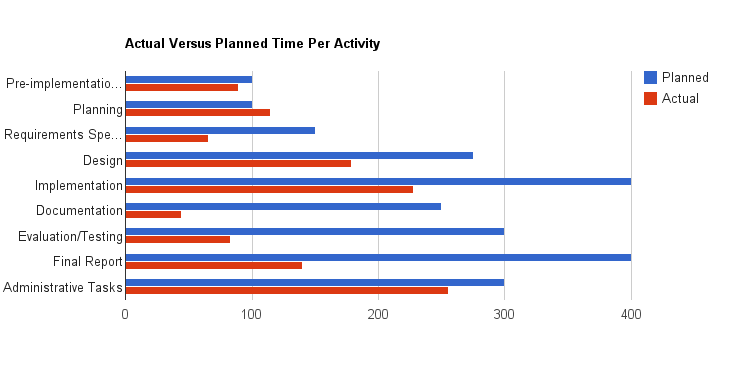
\includegraphics[width = \textwidth]{Evaluation/time_per_activity.png}
    \caption{Actual vs. planned time. By project phase.}
    \label{perActivity}
  \end{figure}
\end{centering}

\begin{centering}
  \begin{figure}
    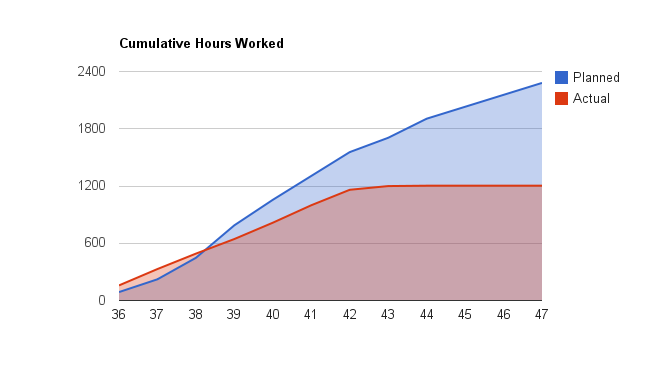
\includegraphics[width = \textwidth]{Evaluation/actual_v_planned_cuml.png}
    \caption{Actual vs. planned time. Cumulative.}
    \label{actualPlannedCuml}
  \end{figure}
\end{centering}

\section{Risks that Occurred}

Referring to the discussion in section~\ref{riskReport}, we can state
in retrospect that few of the risks we anticipated occurred, at least
with major consequences. Some problems occurred building a P3P
parser (risk item 3), causing some initial delays as it took longer time than
anticipated to get the system fully working. This problem was in part
due to some unclear notions in the specification of the dataobjects
storing P3P objects.

Furthermore, the project has not proceded without any conflicts. While
roles and responsibilities were agreed on early on in the project
phase, it turned out that these assignments did not distribute the
workload very evenly.


\section{Course Evaluation - TDT4290}

Finally, we include some notes on how well the objectives of the
course \emph{TDT4290 - Customer Driven Project} itself have been met.